% Add "answers" option to print the answers
\documentclass[addpoints]{exam}

\usepackage[utf8]{inputenc}
\usepackage{calc}
\usepackage{listings}
\usepackage{xcolor}
\usepackage{xspace}

\definecolor{codegreen}{rgb}{0,0.6,0}
\definecolor{codegray}{rgb}{0.5,0.5,0.5}
\definecolor{codepurple}{rgb}{0.58,0,0.82}

\lstdefinestyle{Cstyle}{
    commentstyle=\color{codegreen},
    keywordstyle=\color{magenta},
    numberstyle=\tiny\color{codegray},
    stringstyle=\color{codepurple},
    basicstyle=\ttfamily\small,
    breakatwhitespace=true,         
    breaklines=true,                 
    captionpos=b,                    
    keepspaces=true,                 
    numbers=left,                    
    numbersep=5pt,                  
    showspaces=false,                
    showstringspaces=false,
    showtabs=false,                  
    tabsize=4
}

\lstset{style=Cstyle}

% \makebox[\textwidth]{Name:\enspace\hrulefill}
%  
% \vspace{5mm}
%\makebox[\textwidth]{Instructor’s name:\enspace\hrulefill}

\newcommand{\truefalse}
{		\begin{checkboxes}
			 \choice True
			 \choice False. Explanation: 
		\end{checkboxes}
		\vspace{10pt}
}

\newcommand{\answerspace}[1]
{
	\ifprintanswers
	\else
		\setlength{\mylength}{10pt}%
		%\noindent\rule{\mylength}{20pt}
		%\vspace{\fpeval{1.2*(#1)}}
		\vspace{#1\mylength}
	\fi
}
\newlength{\mylength}

\newcommand\pf[1]{\textcolor{red}{PF: #1}}
\newcommand\am[1]{\textcolor{blue}{AM: #1}}

\newcommand{\answer}[1]{\begin{solution}{#1}\end{solution}}
\newcommand{\ra}{$\rightarrow$\xspace}



\usepackage{color}
\usepackage{minted}
\usepackage{lastpage}
\usepackage{verbatim}
\usepackage{fancyvrb}
\usepackage{graphicx}
\usepackage{float}
\usepackage{algorithm}
\usepackage{listings}
\usepackage{algpseudocode}
\usepackage{tabularx}

\newcommand{\includecode}[2][c]{\lstinputlisting[caption=, escapechar=, language=#1]{#2}<!---->}
\RecustomVerbatimCommand{\VerbatimInput}{VerbatimInput}{}

\renewcommand{\solutiontitle}{\noindent\textbf{Solution sketch: }}

\definecolor{SolutionColor}{rgb}{0.8,0.9,1}


\cfoot{Page \thepage\ of \pageref{LastPage}}

\rhead{Initials: \rule{20mm}{0.4pt}}



%%%%%%%%%%%%%%%%%%%%%%%%%%%%%%%%%%%%%%%%
\begin{document}
\fvset{numbers=left,numbersep=3pt}
\thispagestyle{empty}

\begin{center}
	{\LARGE CS408 Spring 2026 -- Homework 4 (51 points)\\}

	{\Large Deadline: Friday April 10, at \textbf{6pm}\\}

	\vspace{20mm}
\fbox{\fbox{\parbox{5.5in}{\centering
	\begin{itemize}
		\item The Homework is open notes, open book.
		\item No collaboration and no communication of any kind allowed.
		\item Provide complete and clear but concise answers. Justify thoroughly statements where required.
	\end{itemize}
	}}}
\end{center}

\vspace{13mm}
\begin{center}
	\makebox[0.6\textwidth]{
		\combinedgradetable[h][questions]
	}
\end{center}
%\begin{center}\combinedgradetable[h][questions]\end{center}
\vspace{28mm}

\begin{center}
\makebox[\textwidth]{\textbf{Name (please print)}: \rule{100mm}{0.8pt} }
\end{center}

\newpage
\begin{questions}
\question Consider the following C program:

  \begin{minted}{C}
void fun(int a, int b, int c) {
  int x = 100;

  if(a >= 0) {
    x = 50;
  }

  if(b + c > 0) {
    x += c;

    if(x < 70) {
      x += a;
    }
  }
}
\end{minted}

\begin{parts}
\part[10] Provide the execution tree produced by symbolic execution
  for this program. The nodes of this tree should be labelled with the
  corresponding control flow point and the symbolic state\footnote{On
    all of your answers for this question, please name symbolic
    variables using the convention $s_0, s_1, s_2, ...$.} before that
  basic block or condition is executed: using the format L2:
  $[x\mapsto s_1; z \mapsto s_4; \ldots]$. The root of the tree should
  appear at the top of the diagram. The outgoing edges of decision
  nodes should be labelled with the corresponding path conditions, and
  the labels on its left and right subtrees should correspond to the
  true and false branches of the original \texttt{if} statement,
  respectively. To draw a tree, you can either draw the diagram by
  hand or use a tool like \texttt{https://www.yworks.com/yed-live/} or
  \texttt{https://app.diagrams.net/}. If
  you opt for the hand-drawn option, please make sure the image is
  legible: we will deduct points if we can't decipher your
  handwriting.

  %
  \answerspace{10} %
  \answer{
    \begin{center}
      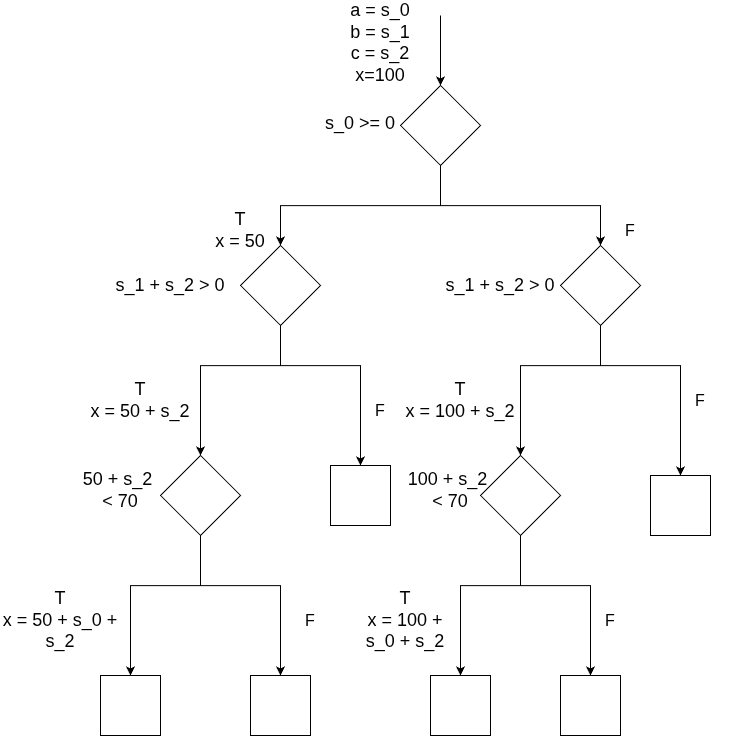
\includegraphics[scale=0.40]{hw4/q1_graph_answer.png}
    \end{center}
  }

  \newpage

\part[2] Please list the path condition corresponding to an execution
  in which the conditions of all three \texttt{if} statements are
  \textbf{true}: (\textbf{true}, \textbf{true}, \textbf{true})
  % \pf{Apply the changes I made here to the other relevant subquestions.}
  % \am{Applied the changes.}
  %
  \answerspace{10} %
  \answer{ %
    ($s_0 \geq 0) \wedge (s_1 + s_2 > 0) \wedge (50 + s_2 < 70)$
  }

\part[2] Please list the path condition corresponding to an execution
  in which the conditions of the first two \texttt{if} statements are
  \textbf{true}, and the last one is \textbf{false}: (\textbf{true},
  \textbf{true}, \textbf{false})
  %
  \answerspace{10} %
  \answer{ %
    $(s_0 \geq 0) \wedge (s_1 + s_2 > 0) \wedge \neg (50 + s_2 < 70)$
    \textbf{OR}
    $(s_0 \geq 0) \wedge (s_1 + s_2 > 0) \wedge (50 + s_2 \geq 70)$
  }

\part[2] Please list the path condition corresponding to an execution
  in which the conditions of the first two \texttt{if} statements are
  \textbf{true}, and the second is \textbf{false}: (\textbf{true}, \textbf{false})

  %
  \answerspace{10} %
  \answer{ %
    ($s_0 \geq 0) \wedge \neg (s_1 + s_2 > 0)$
    \textbf{OR}
    ($s_0 \geq 0) \wedge (s_1 + s_2 \leq 0)$
  }

\part[2] Please list the path condition corresponding to an execution
  in which the conditions of the first \texttt{if} statement is
  \textbf{false}, and those for the other two second are
  \textbf{true}: (\textbf{false}, \textbf{true}, \textbf{true})

  %
  \answerspace{10} %
  \answer{ %
    $\neg (s_0 \geq 0) \wedge (s_1 + s_2 > 0) \wedge (100 + s_2 < 70)$
    \textbf{OR}
    $(s_0 < 0) \wedge (s_1 + s_2 > 0) \wedge (100 + s_2 < 70)$
  }

\part[2] Please list the path condition corresponding to an execution
  in which the conditions of the first \texttt{if} statement is
  \textbf{false}, the next is \textbf{true}, and the last is false:
  (\textbf{false}, \textbf{true}, \textbf{false})

  %
  \answerspace{10} %
  \answer{ %
    $\neg (s_0 \geq 0) \wedge (s_1 + s_2 > 0) \wedge \neg (100 + s_2 < 70)$
    \textbf{OR}
    $(s_0 < 0) \wedge (s_1 + s_2 > 0) \wedge (100 + s_2 \geq 70)$
  }

\part[2] Please list the path condition corresponding to an execution
  in which the conditions of the first two \texttt{if} statements are
  both \textbf{false}: (\textbf{false}, \textbf{false})

  %
  \answerspace{10} %
  \answer{ %
    $\neg (s_0 \geq 0) \wedge \neg (s_1 + s_2 > 0)$
    \textbf{OR}
    $(s_0 < 0) \wedge (s_1 + s_2 \leq 0)$
  }

\end{parts}

\newpage

\question Given the following C program:
% \am {Added the SMT solver comment here and added parantheses to line
% 7}
  \begin{minted}{C}
# include < stdio .h >
# include < math .h >
double bar ( double x , double y , double a , double b ) {
   double result = 0;
   // Program state [2a, 2b]?
   if ( x == y && b > 0) {
     result = (3 * x ) / ( b - a );
   } else {
     x = fmax( x, a );
     a += b ;
     if ( x <= 0) {
       a = a * 3;
      // Program state [2c, 2d, 2e]?
     }
     y = y / 5;
     result = x + y + a + 1;
     // Program state [2f, 2g, 2h]?
   }
   return result ;
 }
\end{minted}

Answer the following questions about the concolic execution of
concrete of \texttt{bar} with the concrete inputs
$[x \mapsto 0, y \mapsto 1, a \mapsto 2, b \mapsto 3]$.

\begin{parts}
\part[2] After the execution of line 4, what is the concrete program state?
  %
  \answerspace{10} %
  \answer{ %
    The concrete program state after L4 is: $x = 0, y = 1, a = 2, b = 3, result=undefined$
  }

\part[2] After the execution of line 4, what is the symbolic program
  state?\footnote{As before, on all of your answers for this question,
    please name symbolic variables using the convention
    $s_0, s_1, s_2, ...$.}  %
  %
  \answerspace{10} %
  \answer{ %
    The symbolic program state after L4 is:
    $x = s_0, y = s_1, a = s_2, b = s_3, result=undefined$
  }

\part[2] After the execution of line 10, what is the concrete program
  state?
  %
  \answerspace{10} %
  \answer{ %
    The concrete program state at L10 is:
    $x = 2, y = 1, a = 5, b = 3, result=undefined$ }
  \vfill

\part[2] After the execution of line 10, what is the symbolic program
  state?
  %
  \answerspace{10} %
  \answer{ %
    To reach line 10 we need $\neg ((s_0 = s_1) \wedge (s_3 > 0))$.
    This gives us the following symbolic state
    $x = max(s_0, s_2), y = s_1, a = s_2 + s_3, b = s_3, result = undefined$
  }

\part[2] What is the path condition after executing line 10?
  %
  \answerspace{10} %
  \answer{ %
    The path condition is $\neg ((s_0 = s_1) \wedge (s_3 > 0))$.
  }

\part[2] After the execution of line 16, what is the concrete program
  state?
  % \pf{Why are these next question using the "for", not "after the execution of line X"? Fix it?}
  % \am {I have added "after the execution of line 16" in the question to be consistent with other parts.}
  %
  \answerspace{10} %
  \answer{ %
    The concrete program state after L16 is: $x = 2, y = 0.2, a = 5, b = 3, result=8.2$
  }

\part[2] After the execution of line 16, what is the symbolic program
  state?
  %
  \answerspace{10} %
  \answer{ %
    $x = max(s_0, s_2), y = s_1 / 5, a = s_2 + s_3 , b = s_3, result = max(s_0, s_2) + s_1 / 5 + s_2 + s_3 + 1$
  }

\part[2] After the execution of line 16, what is the path condition?
  %
  \answerspace{10} %
  \answer{ %
    The path condition is $\neg ((s_0 = s_1) \wedge (s_3 > 0))$.
  }

\part[5] Provide a possible concrete input that concolic execution
  could try after this execution ends.\footnote{You can safely assume
    that the SMT solver understands how \texttt{fmax} works.}  Justify
  your answer in 1-2 sentences.
  %
  \answerspace{10} %
  \answer{ %
    The path condition is $\neg ((s_0 = s_1) \wedge (s_3 > 0))$.
  }
\end{parts}

% \question Given the following program:

% % \am{I have added the SMT solver comment in the question before this one where it should have been. I have also tried to change the program and make the questions more objective.}
% % \pf{Also, this example is not good, this is not that difficult for symbolic execution; use a link traversal example instead. } \pf{We also try to make the 2 next questions more objective.}
% \lstinputlisting{hw4/loop.c}

% \begin{parts}
% \part[5] What features of this program could cause scalability
%   concerns for symbolic execution (if any)? Explain your answer in 1-2
%   sentences.
%   %
%   \answerspace{10} %
%   \answer	{
%     The scalability concern arises from the loop with pointer traversal, since symbolic execution must repeatedly update and maintain the symbolic memory state for each pointer dereference across iterations.
%   }

% % \part[5] Does concolic execution scale better in this example. Explain why.
% %   %
% %   \answerspace{10} %
% %   \answer{ %
% %   Concolic execution scales better in this case because it executes
% %   the program using concrete inputs alongside symbolic tracking. The
% %   concrete values guide the loop and pointer traversal
% %   deterministically, so only one path is explored per run instead of
% %   symbolically expanding every possible heap state.  }

% \end{parts}

\question Please answer the following questions about symbolic/concolic execution.

  \begin{parts}
  \part[4] Please provide 2 advantages of concolic testing over symbolic execution.
    %
    \answerspace{10} %
    \answer{ %
      \begin{itemize}
      \item Handles loops and recursions better by executing
        concretely, avoiding infinite symbolic paths.
      \item Reduces path explosion - explores one concrete path at a
        time instead of all symbolically.
      \item Better handles complex, heap allocated data structures.
      \item Can be adapted to symbolic path conditions without
      \end{itemize}
    }

  \part[4] When generating new concrete inputs during concolic
    execution, what could go wrong if we negated a clause in the path
    condition other than the last one generated? Explain your answer
    in 1-2 sentences.

    % Is the last branch condition of a patch condition in concolic
    % testing negated? Explain your answer.
    %
    \answerspace{10} %
    \answer { The last branch condition in concolic testing is
      typically negated because it is guaranteed to explore a new
      program path.  Negating arbitrarily other clauses in the path
      conditions may not correspond to a path in the program.  }
\end{parts}

% \question[15] Please explain how SMT solvers make use of SAT to determine satisfiability before using theories.
% %
%  \answerspace{10} %
% \answer{ %
% 	Suppose we have a condition such as

%   $$
%     \neg (b + 2 = c) \wedge b + 2 = c \wedge d[c] == \mbox{'\\n'}
%   $$

%   We can see that we use integer, array, and string theories.
%   On inspection we can see that this condition is unsatisfiable because both $b + 2 = c$ and $\neg (b + 2 = c)$ cannot be $\top$ at the same time.

%   A SMT solver is not able to make such an inference.
%   What it does is to replace parts of this condition with symbolic boolean variables.
%   This gives

%   $$
%     \neg b_1 \wedge b_1 \wedge b_2
%   $$

%   where $b_1$ is $b + 2 = c$ and $b_2$ is $d[c] == \mbox{'\\n'}$

%   It uses a SAT solver to check the satisfiability of this equation.
%   Because it is not satisfiable it does not deploy the theories to solve for integers $b$ and $c$ etc and simply returns UNSAT.
% }

\if 0 %%%%%%%%%%%%%%%%%%%%%%%%%%%%%%%%%%%%%%%%%
	\question[10]
	\answerspace{30}
	\answer{ %}

	\question
	\begin{parts}
		\part[6]
		\answerspace{20}
		\answer{ %}

		\part[2]
		%
  \answerspace{10} %
		\answer{ %}

	\end{parts}
\fi %%%%%%%%%%%%%%%%%%%%%%%%%%%%%%%%%%%%%%%%%

	\newpage
	\begin{center}
		[EMPTY PAGE]
	\end{center}

\end{questions}

\end{document}
